\section{Storage--Accuracy Analysis}
\label{sec:compression}
Captured Zigbee network traffic must often be retained to support a-posteriori IoT forensic investigations and long-term monitoring. However, the limited storage resources typically available on edge IoT controllers, combined with the continuous operation of smart home devices, make efficient traffic storage a critical design requirement.

In this section, we analyze the trade-off between storage efficiency and classification accuracy for Zigbee traffic analysis. We compare lossless compression techniques applied directly to raw packet traces with lossy approaches based on compact representations of traffic features. The goal is to quantify how different storage strategies impact the accuracy of downstream traffic classification tasks, and to identify solutions that enable substantial storage reduction without degrading forensic analysis performance.


\subsection{Lossless Compression of Raw Zigbee Packets}
We first evaluate the feasibility of long-term storage of captured Zigbee traffic by retaining raw packet traces in \texttt{.pcap} format and applying standard lossless compression techniques. This approach represents the most straightforward solution for traffic preservation, as it preserves full packet-level information and does not require any modification to the original data representation. At the same time, it establishes an upper bound on storage efficiency achievable without sacrificing information content.
%
Table~\ref{tab:lossless_compression} reports the storage footprint and average bitrate required to store raw Zigbee traffic captured under the two considered network topologies, together with the compression performance achieved using three widely adopted lossless compressors: GZIP, BZIP2, and 7Z-LZMA. These tools were selected due to their protocol-agnostic nature and widespread use in network trace archival.

Without compression, raw Zigbee traffic requires average storage rates of approximately 2.2~kbps and 2.9~kbps for Topology~A and Topology~B, respectively. Here, the storage rate is computed as the total size of the stored \texttt{.pcap} file divided by the corresponding capture duration, yielding an average bitrate over time. These values reflect the cumulative effect of long capture durations and continuous background traffic, despite the low data rate and small packet size characteristic of Zigbee communications.

Applying lossless compression substantially reduces storage requirements. GZIP and BZIP2 achieve comparable performance, reducing the bitrate by approximately 64--65\% across both topologies. Among the evaluated methods, 7Z-LZMA consistently provides the best compression performance, lowering the required storage rate to 657~bps for Topology~A and 768~bps for Topology~B, corresponding to an approximate 3.3× compression ratio relative to uncompressed \texttt{.pcap} files.
% Overall, 7Z-LZMA achieves a compression ratio of approximately 3.3$\times$ relative to the uncompressed \texttt{.pcap} files.

While lossless compression substantially reduces the storage footprint of raw Zigbee traffic, the resulting storage rates can still pose practical constraints in edge-based deployments characterized by limited storage resources and long-term evidence retention requirements. This motivates the exploration of alternative storage strategies based on compact traffic representations and controlled information loss.


% \begin{table*}[]
% \centering
% \begin{tabular}{|l|l|l|l|l|l|l}
% \hline
% \textbf{Device Behaviour} & \textbf{File Name} & \textbf{Duration} & \textbf{Raw size} & \textbf{Raw rate} &  \textbf{7Z-LZMA size} & \textbf{7Z-LZMA rate}}\\ \hline
% Idle & idle.pcap & 5:54:42 & 7137 kbyte & 2.68 kbps &  2121 kbyte & 0.79 kbps\\ \hline
% Physical Interaction& physicalInteraction.pcap& 2:10:25&3206 kbyte& 3.2 kbps & 995 kbyte & 1.01 kbps \\ \hline
% Power Cycling& power.pcap &5:08:10&3334 kbyte&1.44 kbps & 670 kbyte & 0.28 kbps\\ \hline
% Scenario& scenario.pcap &1:31:32&1745 kbyte& 2.54 kbps  & 521 kbyte & 0.75 kbps \\ \hline
% Web Interaction& web\_app.pcap &0:36:22&2326 kbyte& 8.5 kbps & 658 kbyte & 2.31 kbps \\ \hline
% \end{tabular}
% \end{table*}


\begin{table}[h]
    \centering
\caption{Evaluation of Lossless Compression Methods on the ZIOTP2026 PCAP Dataset: Size and Bitrate Across Two Network Topologies}
    \label{tab:lossless_compression}
    \begin{tabular}{lcccc}
    & \multicolumn{2}{c}{Topology A} & \multicolumn{2}{c}{Topology B} \\ \hline
Method & \multicolumn{1}{c}{Size (MB)} & \multicolumn{1}{c}{bps} & \multicolumn{1}{c}{Size (MB)} & \multicolumn{1}{c}{bps} \\
        \midrule
Raw & 6.69 & 2180 & 11.06 & 2880 \\
GZIP & 2.41 & 786 & 3.60 & 937 \\
BZIP2 & 2.36 & 771 & 3.51 & 913 \\
7Z-LZMA & 2.02 & 657 & 2.95 & 768
    \end{tabular}
\end{table}


\subsection{Storage of Traffic Features}
An alternative to storing raw packet traces consists in retaining compact representations of traffic behavior in the form of extracted features. This approach is particularly attractive when the primary objective is traffic analysis rather than packet-level reconstruction, as it eliminates the need for repeated feature extraction during offline processing.

However, unlike IP-based networks, Zigbee environments are characterized by low traffic intensity and small packet sizes. As a consequence, storing raw Zigbee packet traces—especially when combined with lossless compression—may already be relatively storage-efficient. In this setting, feature-based representations are not intrinsically more compact and may require higher storage rates when features are stored using standard high-precision formats.

To clarify this aspect, we consider the window-based feature extraction process described in Section~\ref{sec:data_pre}. Let $N$ denote the number of devices being monitored, $F$ the number of extracted features per window, $b$ the bit width used to encode each feature, and $T$ the window duration. Under these assumptions, the resulting average storage rate can be expressed as
\begin{equation}
    \frac{N \times F \times b}{T} \quad \text{bit/s}.
\end{equation}
This relationship highlights that, in Zigbee-based systems, the storage cost of feature-level representations can easily exceed that of raw packet traces when high-precision feature encodings are adopted.

These considerations indicate that feature-level storage does not automatically yield storage savings in Zigbee networks. Instead, any potential benefit must arise from reducing the precision of the feature representation. To this end, we investigate lossy compression of traffic features through scalar quantization, where each feature is encoded using a reduced number of bits.

Specifically, we generate quantized feature representations using bit depths ranging from 1 to 64 bits per feature. The resulting quantized feature vectors are subsequently compressed using a lossless encoder (7Z-LZMA) to remove residual redundancy. We evaluate two classification scenarios: (i) models trained on unquantized features and tested on quantized features, and (ii) models trained and tested on quantized features using the same bit depth. This analysis allows us to quantify the trade-off between feature precision, storage efficiency, and classification accuracy.



\begin{figure}[ht]
    \centering

    \begin{subfigure}[b]{0.6\textwidth}
        \centering
        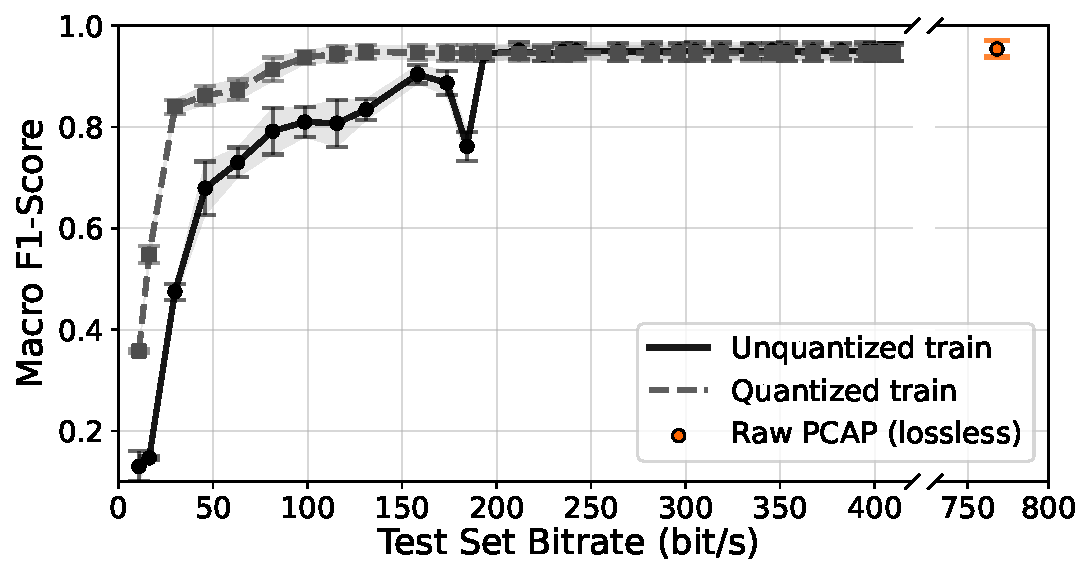
\includegraphics[width=\linewidth]{Figures/dev_type-f1-macro_vs_lzma_bitrate-topoB.pdf}
        \caption{}
        \label{fig:subfig1}
    \end{subfigure}
    \begin{subfigure}[b]{0.6\textwidth}
        \centering
        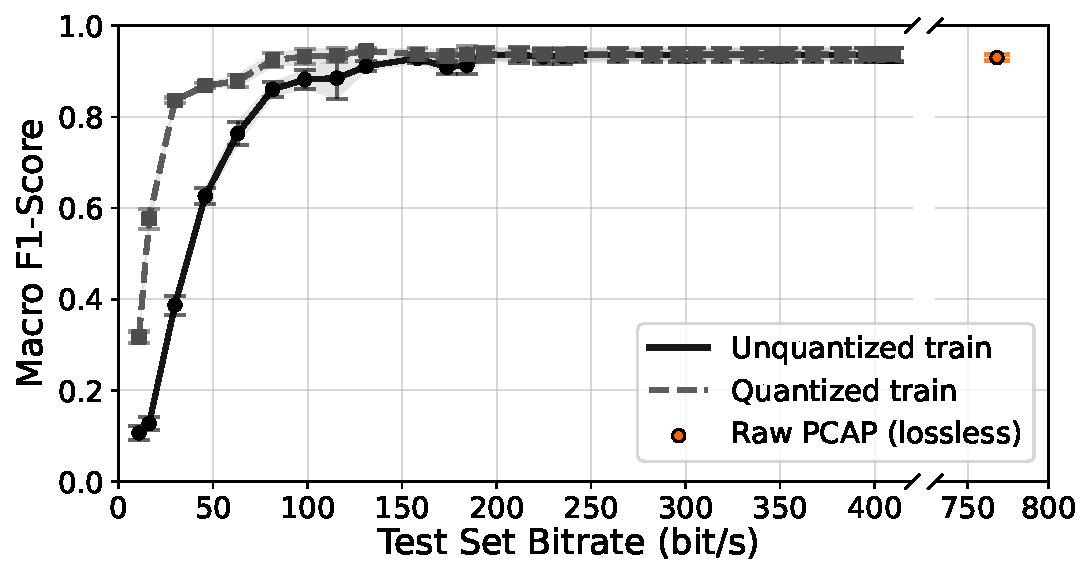
\includegraphics[width=\linewidth]{Figures/dev_name-f1-macro_vs_lzma_bitrate-topoB.pdf}
        \caption{}
        \label{fig:subfig2}
    \end{subfigure}
    \caption{Impact of training set bit-rate on Macro F1 score for (a) device type and (b) individual device identification classification tasks. Results compare two approaches: models trained and tested on quantized data versus models trained on unquantized data but tested on quantized data.}
    \label{fig:quantization_f1_comparison}
\end{figure}

\subsection{Device Type Classification}
Figure~\ref{fig:subfig1} reports the impact of lossy feature compression on device type classification performance, showing the macro F1-score as a function of the average storage bitrate. Results are shown for classifiers trained on unquantized features and evaluated on quantized features, as well as for classifiers trained and tested on quantized representations. For reference, the performance achieved using lossless compression of raw \texttt{.pcap} traces is also indicated.

For both lossy configurations, classification performance improves with increasing bitrate, following a saturating trend. At very low bitrates, aggressive quantization leads to a marked degradation in performance, whereas moderate increases in bitrate rapidly restore classification accuracy.

When the classifier is trained and evaluated on quantized features, macro F1-scores above 0.9 are achieved at bitrates around 100~bit/s, and near-lossless performance is reached at approximately 150--200~bit/s. Beyond this point, further increases in bitrate yield only marginal improvements. In contrast, models trained on unquantized features converge more slowly and exhibit higher variability at intermediate bitrates.

\subsection{Individual Device Identification}
Overall, the performance trends observed for individual device identification are similar to those obtained for device type classification. When the classifier is trained and evaluated on quantized features, performance improves rapidly as the bitrate increases. Macro F1-scores above 0.85 are achieved at bitrates around 80--100~bit/s, while near-lossless performance (macro F1 $\approx$ 0.92--0.94) is reached at approximately 150--200~bit/s. Beyond this range, further increases in bitrate yield marginal performance gains, indicating that most device-specific discriminative information is preserved once a moderate feature precision is retained.

In contrast, models trained on unquantized features and evaluated on quantized representations exhibit slower convergence and higher variability at intermediate bitrates, consistently underperforming the quantized-training configuration. This behavior further confirms that exposing the classifier to quantization effects during training improves robustness to reduced feature precision.


\subsection{Discussion and Implications for IoT Forensics}
The results of this section show that storage strategies for Zigbee traffic impact not only classification accuracy, but also the set of forensic and analytical tasks that can be supported. Lossless storage of raw packet traces preserves complete information and enables the widest range of forensic analyses, including retrospective feature extraction and protocol-level inspection. However, even with state-of-the-art compression, this approach requires storage rates on the order of several hundred bit/s.
Feature-based storage provides a more compact representation at the cost of analytical flexibility. When lossy compression through feature quantization is adopted, storage requirements can be reduced by approximately 4--5$\times$ compared to lossless raw traffic storage, while maintaining near-lossless classification accuracy for both device type classification and individual device identification. Training classifiers directly on quantized features further improves robustness to reduced precision and enables the most storage-efficient operating points.
These gains come with functional limitations. Feature-based representations restrict subsequent analyses to the predefined feature set, preventing packet-level inspection and the extraction of alternative features. As a result, lossy feature compression is well suited for continuous monitoring and classification tasks at the edge, whereas lossless raw traffic storage remains preferable for scenarios requiring full forensic flexibility.
